\documentclass[twocolumn, a4paper, 9pt]{jarticle}

\makeatletter
\def\section{\@startsection{section}{1}{\z@}{2ex plus .2ex minus .2ex}%
  {.5ex plus .2ex minus .2ex}{\large\bfseries}}
\def\thesection{\arabic{section}.}
\def\subsection{\@startsection{subsection}{1}{\z@}{.7ex plus .2ex minus .2ex}%
  {.5ex plus .2ex minus .2ex}{\normalsize\bfseries}}
\def\thesubsection{\arabic{section}.\arabic{subsection}}
\def\thefootnote{\fnsymbol{footnote}}
\makeatother

% Aoyama Lab.
\setlength{\topmargin}{-10mm} % 15mm - 1in
\setlength{\headheight}{5mm}
\setlength{\headsep}{5mm}
\setlength{\oddsidemargin}{-7mm} % 18mm - 1in
\setlength{\evensidemargin}{-7mm} % 18mm - 1in
\setlength{\textheight}{247mm} % 297 - 25(top) - 25(bottom)
\setlength{\textwidth}{174mm} % 210 - 18*2
\setlength{\columnsep}{7mm}

\usepackage{fancyhdr}
\usepackage[english]{babel}
\usepackage[ dvipdfmx]{graphicx}
\usepackage{url}
\usepackage{listings}

\lstset{
  basicstyle={\ttfamily},
  identifierstyle={\small},
  commentstyle={\smallitshape},
  keywordstyle={\small\bfseries},
  ndkeywordstyle={\small},
  stringstyle={\small\ttfamily},
  frame={tb},
  breaklines=true,
  columns=[l]{fullflexible},
  numbers=left,
  xrightmargin=0zw,
  xleftmargin=3zw,
  numberstyle={\scriptsize},
  stepnumber=1,
  numbersep=1zw,
  lineskip=-0.5ex
}

\pagestyle{empty}
\thispagestyle{fancy}
\lhead[]{\fontsize{9pt}{9pt} \sf Keio University Shonan Fujisawa Campus}
\rhead[]{\today}
\cfoot[]{}
\renewcommand{\headrulewidth}{0pt}

\begin{document}

\twocolumn[
  \begin{center}
    {
      {\bf \Large Prediction of Taxi Accidents in Nagoya Using Big Data\\} % 14.4pt
    }
    \vspace{1.5ex}
    {
      \fontsize{10.5pt}{10pt}
      \begin{tabular}{c}
        坂本 嵩$^\dag$  \\
        Shu Sakamoto \\
        71775236
      \end{tabular}
    }
    \vspace{1.5ex}
  \end{center}
]

\insert\footins{
  \noindent
  \small % 9pt
  \begin{tabular}{r p{23em}}
    $^\dag$ & 慶應義塾大学環境情報学部, 〒252-0882 神奈川県藤沢市遠藤5322 \\
  \end{tabular}
}

\section{Introduction}
近年, 社会は目まぐるしく変化しており, その中で個人の多様なライフスタイルが尊重される世の中になりつつある. 特に顕著なものとして働き方があげられ, 大企業のオフィスへと画一的に電車で通勤するスタイルから, 様々な働き場所へ自由な交通手段 (車や自転車など) で向かうスタイルが増えた. しかし車通勤で割けられないのは交通事故であり, 我々は常に死と隣り合わせにいると言っても過言ではない. 特に, 交通事故発生件数一位の都道府県として知られる愛知県では, 1年に39,115件の交通事故が発生した (2017年) \cite{ranking}.\\
悲惨な事故を減らすための有効な手段の一つとして, 頻繁に事故が発生する場所を突き止める箇所を突き止めるという方法がある. ここで本レポートでは, 愛知県名古屋市におけるタクシーの走行データを活用することで, 交通事故が発生しやすい箇所を特定した. 

\section{Data}
データは授業内で配布された\texttt{NagoyaTaxiData}を用いる. 各々の乗務員にはIDが振り分けられており, それぞれに\texttt{SPD[ID].csv}と\texttt{GPS[ID].csv}のデータが存在する. \\
\texttt{SPD[ID].csv}はサンプリングレート120Hzで取得されたスピードデータで, \texttt{時刻,速度,相対距離}が含まれた\texttt{csv}ファイルとなっている. これを以後SPDデータと表記する\\
\texttt{GPS[ID].csv}はサンプリングレート1Hzで取得された位置データで, \texttt{緯度,経度,時刻,測定方位,タリフ状態コード,高速機能}などが含まれた\texttt{csv}ファイルとなっている. これを以後GPSデータと表記する.

\section{解析}
\subsection{目的}
この解析の目的は, 交通事故多発地点を特定することである. ここで, 交通事故が起こりやすい条件を整理する. まず, 交差点付近であることがあげられる. 実に, 交通事故の半数以上が交差点で起きている \cite{ranking}. また, 一方もしくは双方の車両が高速で移動していることも事故の要因になりうる. これは, 飛び出しなどの異変に気がついても高速走行をしていてはブレーキが効かないためである. 以上の理由から, この解析では高速で移動している車が多い交差点付近の地点を探すことを目的とした. 

\subsection{手順}
まず, SPDデータとGPSデータを統合する. これは, 2つのデータのサンプリングレートが違うことを利用し, SPDデータでGPSデータを補間する目的がある. \\
次に, GoogleMap上に車両の速度が0となっている点をプロットする. これにより, 交差点の位置を把握することができる. \\
そして, GoogleMap上に車両が高速で移動している点をプロットする. これにより, 車両が高速で通過しがちは交差点を把握すること, すなわち事故多発地点を把握することができる. 

\subsection{下処理}
\subsubsection{SPDデータ}
SPDデータを目視で確認したところ, 時間順に並んでいなかった. これではGPSデータとの統合を行う際に不便なため, \texttt{sortspd.sh} [\ref{sortspd}] を用いて時刻順にSPDデータを並べ替えた. 

\subsubsection{GPSデータ}
GPSデータには緯度・経度・時刻の他にも様々な情報が含まれているため, これらを取り除く必要がある. また, 緯度・経度情報がデータ独自の方法で表記されているため, これを元に戻す必要がある. 方法は以下の通りである (緯度の場合). 

\begin{enumerate}
  \item 8bitで表記されている情報を2bitずつに分割し, それぞれを8桁の2進数で表示する. e.g.) \texttt{01 02 58 66} → \texttt{00000001 00000010 00111010 01000010}
  \item それぞれの8bitデータの最初の1bitを取り除く. e.g.) \texttt{00000001 00000010 00111010 01000010} → \texttt{0000001 0000010 0111010 1000010}
  \item これを結合する. e.g.) \texttt{0000001 0000010 0111010 1000010} → \texttt{0000001000001001110101000010}
  \item これを4bitごとに区切る. e.g.) \texttt{0000001000001001110101000010} → \texttt{0000 0010 0000 1001 1101 0100 0010}
  \item 4bitデータをそれぞれ16進数に変換する. e.g.) \texttt{0000 0010 0000 1001 1101 0100 0010} → \texttt{0 2 0 9 D 4 2}
  \item これを結合する e.g.) \texttt{0 2 0 9 D 4 2} → \texttt{0209D42}
  \item これを10進数に変換する. e.g.) \texttt{0209D42} → \texttt{2137410}
  \item 10進数データを60000で除算すると, データが復元される \texttt{2137410} → \texttt{35.6235}. 
\end{enumerate}

これを, \texttt{convertTracking.py} [\ref{convertTracking}] を用いて行った. \\

\subsection{SPDデータとGPSデータの統合}

上記の方法で下処理が完了したSPDデータとGPSデータを, \texttt{spdgps.py} [\ref{spdgps}] を用いて統合する. このプログラムでは, SPDデータを60Hzにダウンサンプリングした上で, SPDデータの速度情報を用いてGPSデータを補間する. 最終的にはサンプリングレート60Hzの速度情報と位置情報を持ったSPDGPSデータが出力される. また, SPDデータもしくはGPSデータが存在しない点に関しては取り除く. その他細かい手順はプログラム及びそのコメントに譲る. \\
また, これらのデータを \texttt{cat SPDGPS*.csv > all.csv} コマンドを用いて一つのファイルに統合する. 

\subsection{外れ値の除去}

以上の手順で統合した\texttt{all.csv}をプロットしたのがFig. \ref{fig:raw} である. 図の左上に存在する外れ値の影響で, プロットがみにくくなってしまっている. これを解決するため, \texttt{denoise.py} [\ref{denoise}] で一定の範囲内に収まらないプロットは除去した (Fig. \ref{fig:denoise}). 

\begin{figure}[htbp]
  \begin{center}
    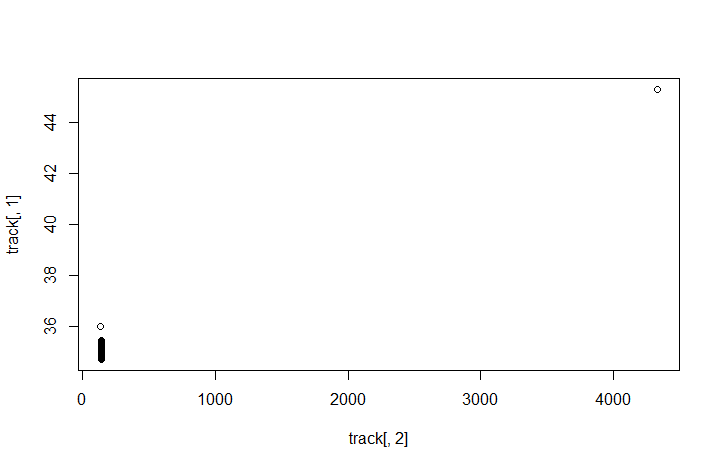
\includegraphics[clip,width=8cm]{images/allplot_raw.png}
    \caption{外れ値を含んだデータのプロット.}
    \label{fig:raw}
  \end{center}
\end{figure}

\begin{figure}[htbp]
  \begin{center}
    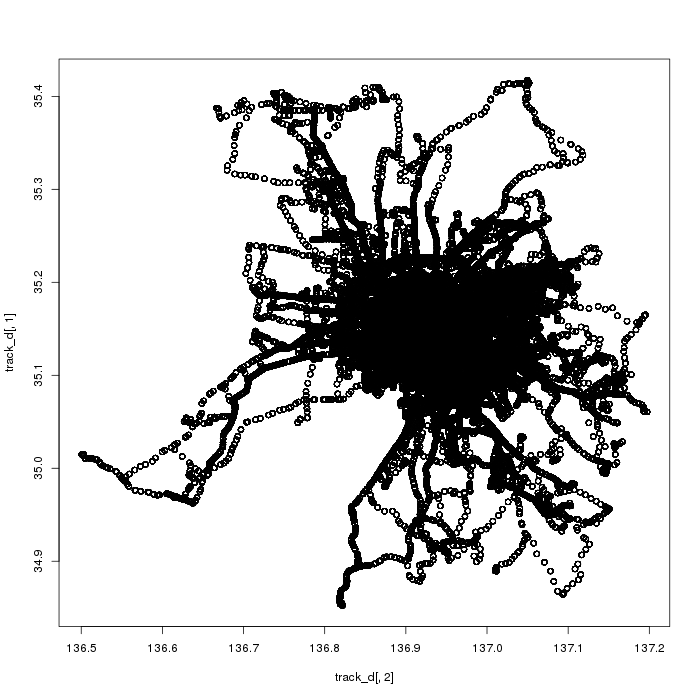
\includegraphics[clip,width=8cm]{images/allplot_denoise.png}
    \caption{外れ値を除去したデータのプロット.}
    \label{fig:denoise}
  \end{center}
\end{figure}

\subsection{交差点のプロット}

\subsection{高速走行箇所のプロット}

\subsection{交通事故多発地点の特定}

\section{まとめ}

以上の解析を用いて交通事故多発地点と思われる場所を探すことができた. また, これらの地点は実際の交通事故多発地点とある程度一致した. 今後の解析として, 場所情報のみならず地形や建物の情報, つまり見通しなども考慮することでより正確な予測をしたい. 

\bibliographystyle{jplain}
\bibliography{report}

\onecolumn

\begin{lstlisting}[caption=sortspd.sh, label=sortspd]
  # SPD.csvを時刻順に処理する
  # ./sortspd SpeedData/*
  path=$1
  files=`find $path -maxdepth 1 -type f -name SPD*.csv`
  
  for file in $files;
  do
      newfile="${file:0:-4}_sorted.csv"
      echo $newfile
      sort -t , -k 1 $file > $newfile
  done  
\end{lstlisting}

\begin{lstlisting}[caption=convertTracking.py, label=convertTracking]

  # python convertTracking.py TrackingData/
  import csv
  import sys
  import glob
  
  
  def getDegree(s):
      v0_bin = format(int(s[0:2], 16), 'b').zfill(8)
      v1_bin = format(int(s[2:4], 16), 'b').zfill(8)
      v2_bin = format(int(s[4:6], 16), 'b').zfill(8)
      v3_bin = format(int(s[6:8], 16), 'b').zfill(8)
  
      bin_bit = v0_bin[1:] + v1_bin[1:] + v2_bin[1:] + v3_bin[1:]
  
      hex_int = ''
      for i in range(7):
          hex_int += str(format(int(bin_bit[i*4:i*4+4], 2), 'x'))
  
      dec_int = int(hex_int, 16)
  
      deg = dec_int / 60000.0
  
      return str(deg)
  
  
  def getISO8601(s):
      ye = int(s[0:2]) + 2000
      mo = int(s[2:4])
      da = int(s[4:6])
      h = int(s[8:10])
      m = int(s[10:12])
      s = int(s[12:14])
      return ("{:04}-{:02}-{:02}T{:02}:{:02}:{:02}+09:00".format(ye, mo, da, h, m, s))
  
  
  path = sys.argv[1]
  
  files = glob.glob(path + "GPS*.csv")
  
  for file in files:
      outs = [["lon", "lat", "time", "orientation", "tariff", "high"]]
  
      csv_file = open(file, "r", encoding="shift_jis")
      f = csv.reader(csv_file, delimiter=",", lineterminator="\r\n",
                     quotechar='"', skipinitialspace=True)
  
      print(file)
  
      for row in f:
          if row == []:
              continue
          lon = getDegree(row[0][0:8])
          lat = getDegree(row[0][8:16])
          time = getISO8601(row[0][16:30])
          orientation = str(int(row[0][30:34], 16))
          tariff = row[1]
          high = row[2][0:2]
          out = [lon, lat, time, orientation, tariff, high]
          outs.append(out)
  
      outfile = file[:-4] + "_conv.csv"
  
      with open(outfile, 'w', encoding="utf_8") as ff:
          writer = csv.writer(ff, lineterminator='\n')  # 改行コード(\n)を指定しておく
          writer.writerows(outs)  # 2次元配列も書き込める
\end{lstlisting}  

\begin{lstlisting}[caption=spdgps.py, label=spdgps]
  import csv, sys, glob, datetime, pprint

  ## functions
  
  def time_spd2gps(tstr: str) -> str:
      '''
      SPDデータの時刻を, GPSデータの表記に合わせる. 
      Input: 
          tstr: SPDデータの時刻. str型. 
      Output:
          GPSデータ表記の時刻. str型. 
      '''
      ye = tstr[0:4]
      mo = tstr[5:7]
      da = tstr[8:10]
      h = tstr[11:13]
      m = tstr[14:16]
      s = tstr[17:19]
  
      return ("{}-{}-{}T{}:{}:{}+09:00".format(ye, mo, da, h, m, s))
  
  def sameride(tstr1: str, tstr2: str) -> bool:
      '''
      2つ時刻データ (tstr1, tstr2) が1秒より離れていないか確かめる (データの切れ目をdetectする).
      Input:
          tstr1: 1つ目の時刻データ. str型.
          tstr2: 2つ目の時刻データ. str型.
      Output:
          Bool型. tstr1とtstr2が1秒より離れていなければTrue.それ以外はFalse.
      '''
      t1 = datetime.datetime(year=int(tstr1[0:4]), month=int(tstr1[5:7]), day=int(tstr1[8:10]),
                             hour=int(tstr1[11:13]), minute=int(tstr1[14:16]), second=int(tstr1[17:19]))
      t2 = datetime.datetime(year=int(tstr2[0:4]), month=int(tstr2[5:7]), day=int(tstr2[8:10]),
                             hour=int(tstr2[11:13]), minute=int(tstr2[14:16]), second=int(tstr2[17:19]))
      diff = t2 - t1
      return diff.total_seconds() < 2
  
  ## init
  path_gps = sys.argv[1]  # nagoya/TrackingData/
  path_spd = sys.argv[2]  # nagoya/SpeedData/
  path_dst = sys.argv[3]  # nagoya/TrackingSpeedData/
  
  files_gps = glob.glob(path_gps + "GPS*_conv.csv")
  files_spd = glob.glob(path_spd + "SPD*_sorted.csv")
  
  ## main
  for file_spd in files_spd:
  
      idstr = file_spd[-14:-11]
      file_gps = path_gps + "GPS" + idstr + "_conv.csv"
      file_dst = path_dst + "GPSSPD" + idstr + ".csv"
  
      if file_gps not in files_gps:
          continue
  
      print("reading {}...".format(file_spd))
  
      # spd の読み込み
      # 2013/08/01 08:53:01.0,0,0
      data_spd = []
      times_spd = []
      with open(file_spd, 'r') as f:
          reader = csv.reader(f)
          for row in reader:
              if row == []:
                  continue
              if row[0][-1] == '5': # ダウンサンプリング
                  continue
  
              row[0] = time_spd2gps(row[0])
              data_spd.append(row)
              times_spd.append(row[0])
  
      print("reading {}...".format(file_gps))
  
      # gps の読み込み
      # ヘッダあり, 35.130516666666665,136.98396666666667,2013-07-31T20:32:15+09:00,2661,00,00
      data_gps = []
      times_gps = []
      last_row = []
      with open(file_gps, 'r') as f:
          reader = csv.reader(f)
          header = next(reader)
          for row in reader:
              #  もしgpsの時刻がspdになければ, 行を削除
              # そうでなければ二次元配列data_gpsに格納
              # 時刻をtime_gpsに格納
              if row == []:
                  continue
  
              time_gps = row[2]
              if not time_gps in times_spd:
                  continue
              if row==last_row:
                  # print(row)
                  continue
              times_gps.append(time_gps)
              data_gps.append(row)
              last_row = row
  
      # print("data_spd")
      # pprint.pprint(data_spd[:10], width=50)
      # print("data_gps")
      # pprint.pprint(data_gps[:10], width=50)
  
      data_spd_btw = []           # GPS時刻の間にあるSPDデータ
      spd_vel = []                # SPD時刻で補間する時間窓内の速度
      gps_t1 = []                 # SPD時刻で補間されるGPS時刻の開始地点
      gps_t2 = []                 # SPD時刻で補間されるGPS時刻の終了地点
      idx_gps = 0                 # 読んでいるGPSの行を知るためのカウンター
      gps_ndata = len(data_gps)   # GPSデータの総数
      spd_ndata = len(data_spd)   # SPDデータの総数
      data_dst = []               # file_dstに保存する2次元配列
      samerideFlag = True
  
      print("interpolating gps with spd...")
  
      for idx_spd, datum_spd in enumerate(data_spd):
  
          # データが最後に到達したら処理を終える
          if idx_gps == gps_ndata-1 or idx_spd == spd_ndata-1:
              print("\ngps_ndata: {}\nidx_gps: {}\nspd_ndata: {}\nidx_spd: {}"\
                      .format(gps_ndata, idx_gps, spd_ndata, idx_spd))
              break
  
          # if idx_spd%100000 == 0: print("\nidx_spd: ",str(idx_spd))
  
          # GPS時刻==SPD時刻まで, (間の) SPD時刻をストックしておく
          time_spd = datum_spd[0]
          time_spd_nxt = data_spd[idx_spd+1][0]
          time_gps = data_gps[idx_gps][2]
  
          if time_spd != time_gps and sameride(time_spd, time_spd_nxt):
              # print("hi, time_spd{}, time_gps{}".format(time_spd, time_gps))
              data_spd_btw.append(datum_spd)
              continue
  
          # データの切れ目は切り捨てる
          # 終末の切れ端
          if not sameride(time_spd, time_spd_nxt):
              print("not sameride, idx is {}, data is {}".format(idx_spd, datum_spd))
              # print("previous time_gps: {}\ntime_gps: {}\nnext time_gps: {}\ntime_spd: {}\n".\
                      # format(data_gps[idx_gps-1][2], time_gps, data_gps[idx_gps+1][2], time_spd))            
              data_spd_btw = []
              samerideFlag = False
              continue
          # 始点の切れ端
          if time_gps==time_spd and not samerideFlag:
              print("not samerideFlag, idx is {}, data is {}\n".format(idx_spd, datum_spd))
              # print("time_gps: {}\nnext time_gps: {}\ntime_spd: {}\n\n".format(time_gps, data_gps[idx_gps+1][2], time_spd))
              data_spd_btw = []
              idx_gps += 1
              samerideFlag = True
              continue
  
          # 最初のGPS時刻は切り捨てる
          if idx_gps == 0:
              data_spd_btw = []
              idx_gps += 1
              continue
  
          # 補間処理
          # 終点のspdも追加する
          data_spd_btw.append(datum_spd)
  
          gps_t1 = data_gps[idx_gps-1]
          gps_t2 = data_gps[idx_gps]
          vels_spd_btw = [int(datum_spd_btw[1]) for datum_spd_btw in data_spd_btw]
  
          vel_total = sum([int(vel_spd_btw) for vel_spd_btw in vels_spd_btw]) + 1 # to avoid div0
          lon_t1 = float(gps_t1[0])
          lon_t2 = float(gps_t2[0])
          lat_t1 = float(gps_t1[1])
          lat_t2 = float(gps_t2[1])
          lon_diff = lon_t2-lon_t1
          lat_diff = lat_t2-lat_t1
  
          # velによってlon,latを補間する
          # lon,lat,time,tariff,vel
          for datum_spd_btw in data_spd_btw:
              t = datum_spd_btw[0]
              vel = int(datum_spd_btw[1])
              lon = lon_t1 + lon_diff * vel/vel_total
              lat = lat_t1 + lat_diff * vel/vel_total
              tariff = gps_t1[4]
              datum_dst = [str(lon), str(lat), t, tariff, str(vel)]
              data_dst.append(datum_dst)
  
          data_spd_btw = []
          idx_gps += 1
      
      # ファイルに書き込み
      with open(file_dst, 'w', encoding="utf_8") as ff:
          writer = csv.writer(ff, lineterminator='\n')  # 改行コード(\n)を指定しておく
          writer.writerows(data_dst)  # 2次元配列も書き込める
\end{lstlisting}

\begin{lstlisting}[caption=denoise.py, label=denoise]
  import csv
  import sys
  
  path = sys.argv[1]
  
  file = path + "all.csv"
  newfile = path + "all_denoise.csv"
  outs = list()
  
  csv_file = open(file, "r", encoding="utf_8")
  f = csv.reader(csv_file, delimiter=",", lineterminator="\r\n", quotechar='"',
                 skipinitialspace=True)
  
  for row in f:
      if not 136.4 < float(row[1]) < 137.5:
          continue
      if not 34.6 < float(row[0]) < 35.6:
          continue
      out = row
      outs.append(out)
  
  with open(newfile, 'w') as ff:
      writer = csv.writer(ff, lineterminator='\n')  # 改行コード(\n)を指定しておく
      writer.writerows(outs)  # 2次元配列も書き込める
\end{lstlisting}

\end{document}